\documentclass[a4paper,12pt]{article}
\usepackage[MeX]{polski}
\usepackage[utf8]{inputenc}
\usepackage{graphicx}

%opening
\title{Tabele i obrazki}
\author{Łukasz Szymborski}
\date{31 października 2017}

\begin{document}
%
\maketitle

\begin{abstract}
Dokument do ćwiczeń z tabel i obrazków.
\end{abstract}
%
\centering Dowolny tekst zawierający cytat ,,polski'' i ``anglosaski''.
%
\begin{table}[h]
\centering
\begin{tabular}{c|l|l}
Model & Taktowanie & Data produkcji \\
\hline
i5-650 & $3,20$GHz & I 2010 \\
\hline
i5-660 & $3,33$GHz & II 2010 \\
\hline
i5-661 & $3,33$GHz & I 2010 \\
\hline
i5-670 & $3,46$GHz & I 2010 \\
\hline
i5-680 & $3,60$Ghz & II 2010 \\
\end{tabular}
\caption {Tabela testowa na rzecz ćwiczeń z artykułu "Intel Core i5"}
\end{table}

\begin{figure}[h]
\centering
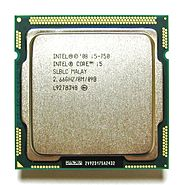
\includegraphics[bb=0 0 185 185]{Intel_Core_i5.jpg}
\caption{Zdjęcie procesora na rzecz ćwiczeń}
\label{fig:cpu}
\end{figure}
%
Zdjęcie \ref{fig:cpu} przedstawia przykład procesora i5.
%
\begin{flushleft}
Intel Core i5 jest wariantem serii Intel Core i7. i7 od i5 zazwyczaj różni się podwojoną liczbą wątków oraz zwiększeniem pamięci cache. Serie Core i5 posiadają zintegrowany kontroler pamięci RAM, zintegrowany kontroler karty graficznej PCI Express oraz kontroler Direct Media Interface do~komunikacji z chipsetem. Jego gniazdem są LGA 1150, LGA 1155, LGA 1156 oraz najnowsze LGA 1151.

\textasciitilde
\end{flushleft}
%
\end{document}